\section{Оршил хэсэг} 

\subsection{Зорилго} 

\begin{frame}
\frametitle{Зорилго}
\begin{block}{}
\justifying
Камерын хэрэглээ нь судалгааны ажил болон хувийн хэрэглээнд жижиг өрөө тасалгаанд хэрэглэх боломжтой байна. Дүрс бичлэгтэй холбоотой тохиргоо, туршилтыг хийж боломжтой хяналтын камерыг угсрах болон камерын системийг бүтээхэд төслийн зорилго оршино.
\end{block}
\end{frame}

\subsection{Зорилт} 

\begin{frame}
\frametitle{Зорилт}
\begin{itemize}
\item Веб интерфейстэй 
\item Бүртгэлтэй хэрэглэгч нэвтэрдэг
\item Алсаас шууд бичлэг үзэх (live stream)
\item Бичлэг болон зурган байдлаар хадгалах
\item Хадгалж байгаа файлыг татдаг
\item Тохиргоог харах болон өөрчилдөг 
\end{itemize}
\end{frame}



\section{Ерөнхий хэсэг} 

\subsection{Хяналтын камер} 
\begin{frame}
\frametitle{Камер}
	\begin{figure}[htp]
	\centering
	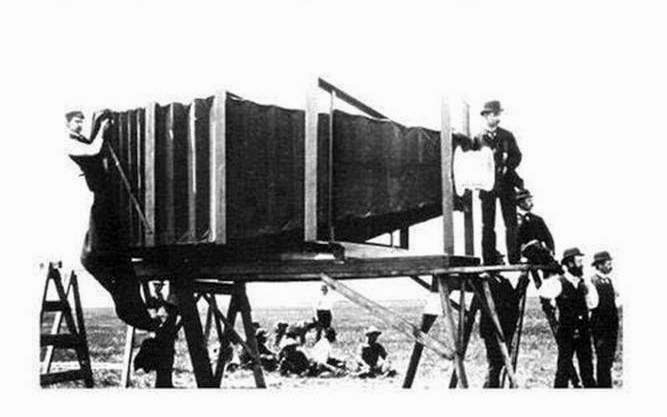
\includegraphics[width=7cm,height=5cm ]{figures/first.jpg}
	\caption{ Дэлхий дээрх анхний камер 1900 он}
	\label{fig:lion}
	\end{figure}
	
	
\end{frame}
\begin{frame}
\frametitle{Камер}
	\begin{figure}[htp]
	\centering
	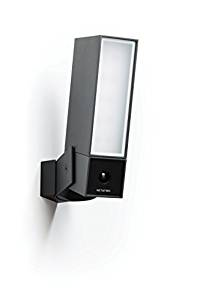
\includegraphics[width=3cm,height=5cm ]{figures/last.jpeg}
	\caption{ 2017 оны хамгийн шилдэг камер NETATMO}
	\label{fig:lion}
	\end{figure}
	
	
\end{frame}





\subsection{Төхөөрөмж} 
\begin{frame}
\frametitle{Төхөөрөмж}
	\begin{figure}[htp]
	\centering
	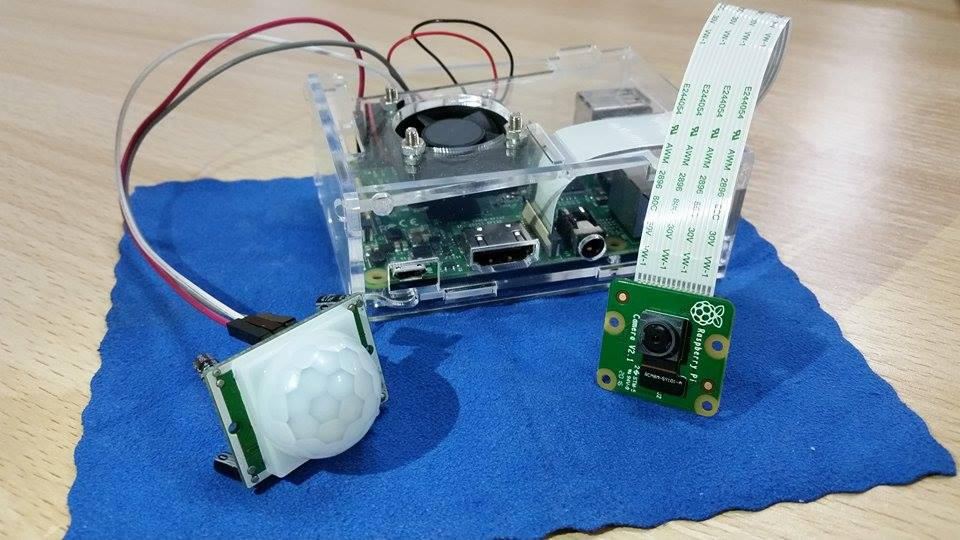
\includegraphics[width=\textwidth,height=6cm ]{figures/mycam.jpg}
	\caption{ Манай камер}
	\label{fig:lion}
	\end{figure}
 \end{frame}
 
 
\begin{frame}
\frametitle{Төхөөрөмж}
	\begin{figure}[htp]
	\centering
	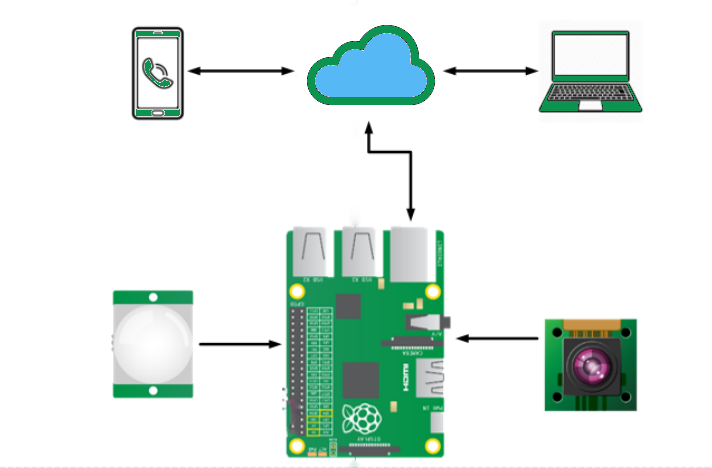
\includegraphics[width=\textwidth,height=6cm ]{figures/device.png}
	\caption{Ерөнхий холболт}
	\label{fig:lion}
	\end{figure}
 \end{frame}

\begin{frame}
\frametitle{Хөдөлгөөн мэдрэгч}
	\begin{figure}[htp]
	\centering
	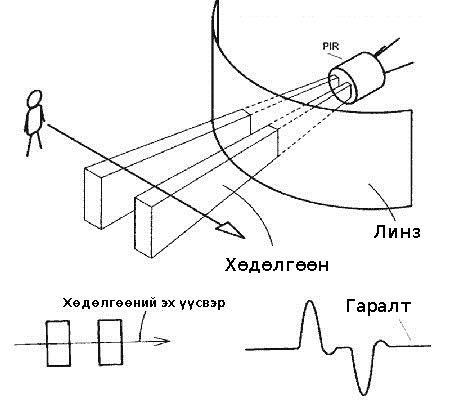
\includegraphics[width=\textwidth,height=6cm ]{figures/motionexm.png}
	%\caption{Ерөнхий холболт}
	\label{fig:lion}
	\end{figure}
 \end{frame}
\subsection{Хяналтын камерын системийн хөгжүүлэлт} 
\begin{frame}
\frametitle{ Блок схем}
	\begin{figure}[htp]
	\centering
	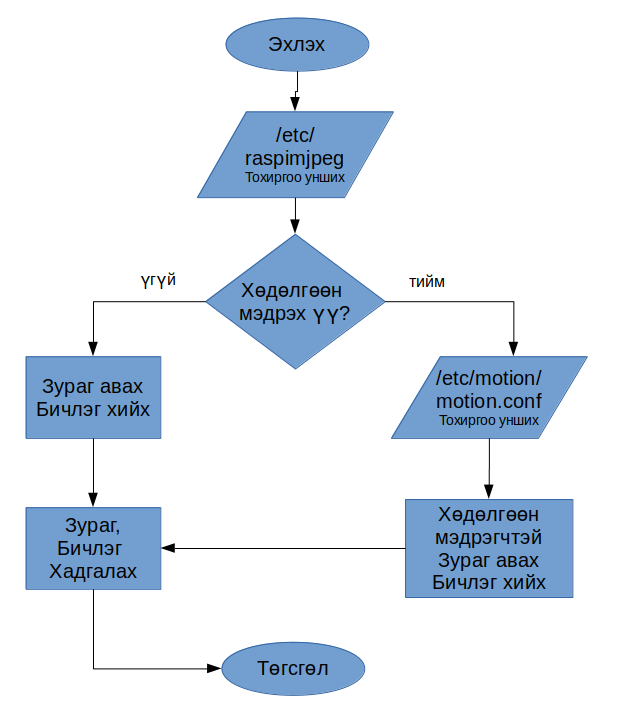
\includegraphics[width=5cm,height=7cm ]{figures/block.jpg}
	%\caption{Ерөнхий холболт}
	\label{fig:lion}
	\end{figure}
 \end{frame}

 
\begin{frame}
\frametitle{206-р ангийн хөдөлгөөнтэй дохио}
\begin{center}
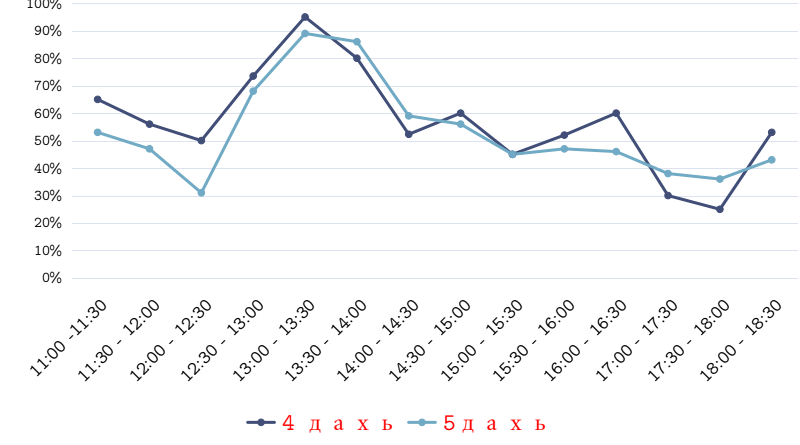
\includegraphics[width=8cm,height=5cm ]{figures/dig.png}
\end{center}

\end{frame}

\subsection{ Stream хийх хэсэг} 
\begin{frame}
\frametitle{HTML хэсэг}
\html
\end{frame}

\begin{frame}
\frametitle{Javascript хэсэг}
\js
\end{frame}
 
\begin{frame}
\frametitle{Өгөгдөл авах хэсэг}
\php
\end{frame}
 

\section{Дүгнэлт} 
\begin{frame}
\frametitle{Дүгнэлт}
\begin{block}{}
\justifying
Raspbian үйлдлийн системийн raspimjpeg, motion гэсэн 2 программын хэргэлэн ажилдаг. Apache сервер дээр ажилж байгаа веб хуудснаас linux-ын коммандыг дуудан ажилуулж байна. Raspberry руу ip сүлжээгээр холбогдон шууд бичиж байгаа бичлэг үзэж болж байгаа. Хадгалж байгаа бичлэг болон зургийг холбогдсон хэрэглэгч татаж авах боломжтой. 
\end{block}

\end{frame}